% !TEX root = ../Dissertation.tex
% !TEX spellcheck = en_US

% THIS IS THE SECOND CHAPTER %
\noindent 

The following describes describes the failure distribution, commonly applied failure and repair rates to the backbone networks.  

\section {Introduction}
Analysis of survivability begins from introducing failures in the network and test its performance against realistic failure scenarios. Backbone networks are usually well-engineered and adequately provisioned, leading to very low packet losses and negligible queueing delays. This robust network design is one of the reasons why the occurrence and impact of failures in these networks have received little attention[16]. However, these reliability measures have little to guard links from accidental failures due to earthquake, terrorist attack, digging works etc.,. An in-depth understanding of reasons for such failures can only be known if vendors reveal the failure data of their network. Unfortunately, the lack of failure data from operational networks has further limited the investigation of failures in backbone networks. Also, ESnet did not reveal any such failure data about the network and this forces to consider the most common scenarios of accidental link failures. In most of the networks, 25\% of the failures in the network is due to the scheduled maintenance activities. This research considered only unplanned link failures due to fiber cuts and amplifier failures which may lead to unexpected connection interruption. 

\section {Failure characteristic and distribution}
%figure 4.1

\begin{figure}[hbt!]
\centering
\includegraphics[width=12cm, height=8cm, page=18]{fig16.png}
\caption{Bathtub Curve[bathtubcurve]}
\label{fig:bathtubCurve}
\end{figure}

The figure 4.1 is called the bathtub curve and it does not depict the failure of a single item, but describes the relative failure rate of an entire population of products over time. It is common to assume Weibull distribution[www.weibull.com] for modeling failures for practical applications. This is because of the adaptability of this distribution to the bathtub curve. The curve is divided in to three regions and each of these regions behaves differently. Any equipment in its early period has decreasing or zero failure rates because new items are less likely to fail often. This corresponds to the decreasing part of the bathtub curve. Later, failure rate remains constant in normal useful life. At this period, failure is completely random in time and even the considered relative sample.  Here the failure rates are constant. This corresponds to the flat line of the bathtub curve. The third and the final region is 'wear-out' region. Here, the failure rates increase to infinity and the components need to be replaced. This is the rightmost increasing part of the curve.
	
\indent All three regions can be easily modeled with Weibull. In fact, the flat region of the curve exhibits exponential distribution. This is the region where the failures are random and can be used to model accidental failure scenarios. That said, it is not appropriate to consider other regions of bathtub curve unless more data on failures can be known. If the links are assumed to experience accidental failures due to external influence, it safe to consider the middle region of bathtub curve. This research does not consider deliberate failures or failure of links due to aging. Equipment vendors can model their own failure rate curve like bathtub curve and can set threshold on replacements based on the demands and requirements of the customer. 

\indent The work in [17] explores the application of Weibull distribution and fits it to the network-wide time between failures. The work in [18] investigated UNINETT IP backbone on a per-link basis and fits the up time of these links to well-known distributions. It is important to consider that in [18], the links are characterized based on the length. For example, the short, medium distance links are fitted to Weibull distribution with shape parameter less than 1 whereas the long-distance links could be modeled with Gamma distribution [www.itl.nist.gov]. To derive these failure data, the vendors should outsource the information and an accurate modeling can be possible by fitting each link to its corresponding distribution. But in order to do this, the location and number of failures of link should be observed for a reasonable period of time. The authors of [17], [18] also warned to not to blindly apply these parameters to any other network as it may lead to a deception in the failure analysis. Another option would be assume Poisson distribution as the time between two failures in the same link is independent to each other. This is very appropriate to model the accidental failures caused in the link. This is because accidents int he same link at different times have no relation to each other. Hence, this research assumes arrival of failure follows poisson distribution[21].  

	 Many researchers from [19] [20] [21] have found that the failure of links is directly proportional to the distances and that failures of each links are independent to each other. In fact, [19] has given the failure rates and repair rates of the links based on their installation types, which will be discussed in the following section. 
	
\section{Failure and Repair Rates}	

In reliability engineering, one should be very familiar with few terms.		

\begin{enumerate}[label=(\alph*),leftmargin=*]
\item\textit{MTTR or Downtime}\\
	The average time that it takes to repair a failed component,
\item\textit{MTBF or Uptime}\\
	The average time that it takes for a link to fail
\item\textit{Availability = (MTBF-MTTR)/MTBF}
\item\textit{FIT (failure-in-time)}\\
The term FIT is defined as a failure rate of 1 per billion hours.
\end{enumerate}

Chapter 1 describes the basic reliability parameters to model the failure of a product. These parameters are FIT and MTTR. This research fits these values to link failures from extensive review of  [22], [23], [24], [25], [26] [27] and derives approach based on majority consensus of these authors. Since not all ESnet links are buried (some of the them goes under the sea), the FIT's for buried links were picked up from [22], [26], overseas from [22] and amplifiers from [23], [27]. The concluded final values are tabulated as follows.

%Table 4.1 ESNet link summary
\begin{table}[!htbp]
\centering
\caption{Summary of Failure Rate assumptions based on its geographical location}
 	\begin{tabular}{|c|c|c|c|}
	\hline\hline
	\textbf{Installation Type of Link} & \textbf{FIT/km} & \textbf{Amplifier FIT} & \textbf{MTTR (in hrs)}\\
	\hline
	Buried&114&2850&20\\
	Overseas&21.55&2850&450\\
	\hline
	\end{tabular}
\end{table}

 Usually, amplifiers are assumed to be located every 100 km. Once the FIT of a link is known, the MTBF can be calculated as follows,

MTBF = 1000000000/ FIT x Total link length

Total link length (includes amplifier failures) = ((Amplifier FIT/Link FIT) x (Link distance/Number of amplifiers)) + link distance.

Using this formula, the MTBF can be calculated for all the links as shown in the topology. 
%Fig. 4.2 ESNet Topology with MTTR and MTTF

\begin{figure}[hbt!]
\centering
\includegraphics[width=15cm, height=10cm, page=18]{fig17.png}
\caption{Augmented ESnet Topology with distance/MTTF}
\label{fig:esnetTopo}
\end{figure}
%Table 4.2 Link counts based on installation type
\begin{table}[!htbp]
\centering
\caption{Number of links based on geographical location}
 	\begin{tabular}{|c|c|}
	\hline\hline
	\textbf{Type} & \textbf{Number of links}\\
	\hline
	Buried&66\\
	Overseas&6\\
	\hline
	\end{tabular}
\end{table}


